\section{Week 2 - Natural Language Processing \& Word Embeddings}
\subsection{Introduction to Word Embeddings}

\subsubsection
So far we were repsenting words with vocabulary, and 1-hot representation (binary vector).
This treats each word as a thing in itself and does not allow the algorithm to learn relationships between words. This is because the in-product between any word is 0, it does not know that orange and apple are similar words.

\begin{figure}[H]
\centering
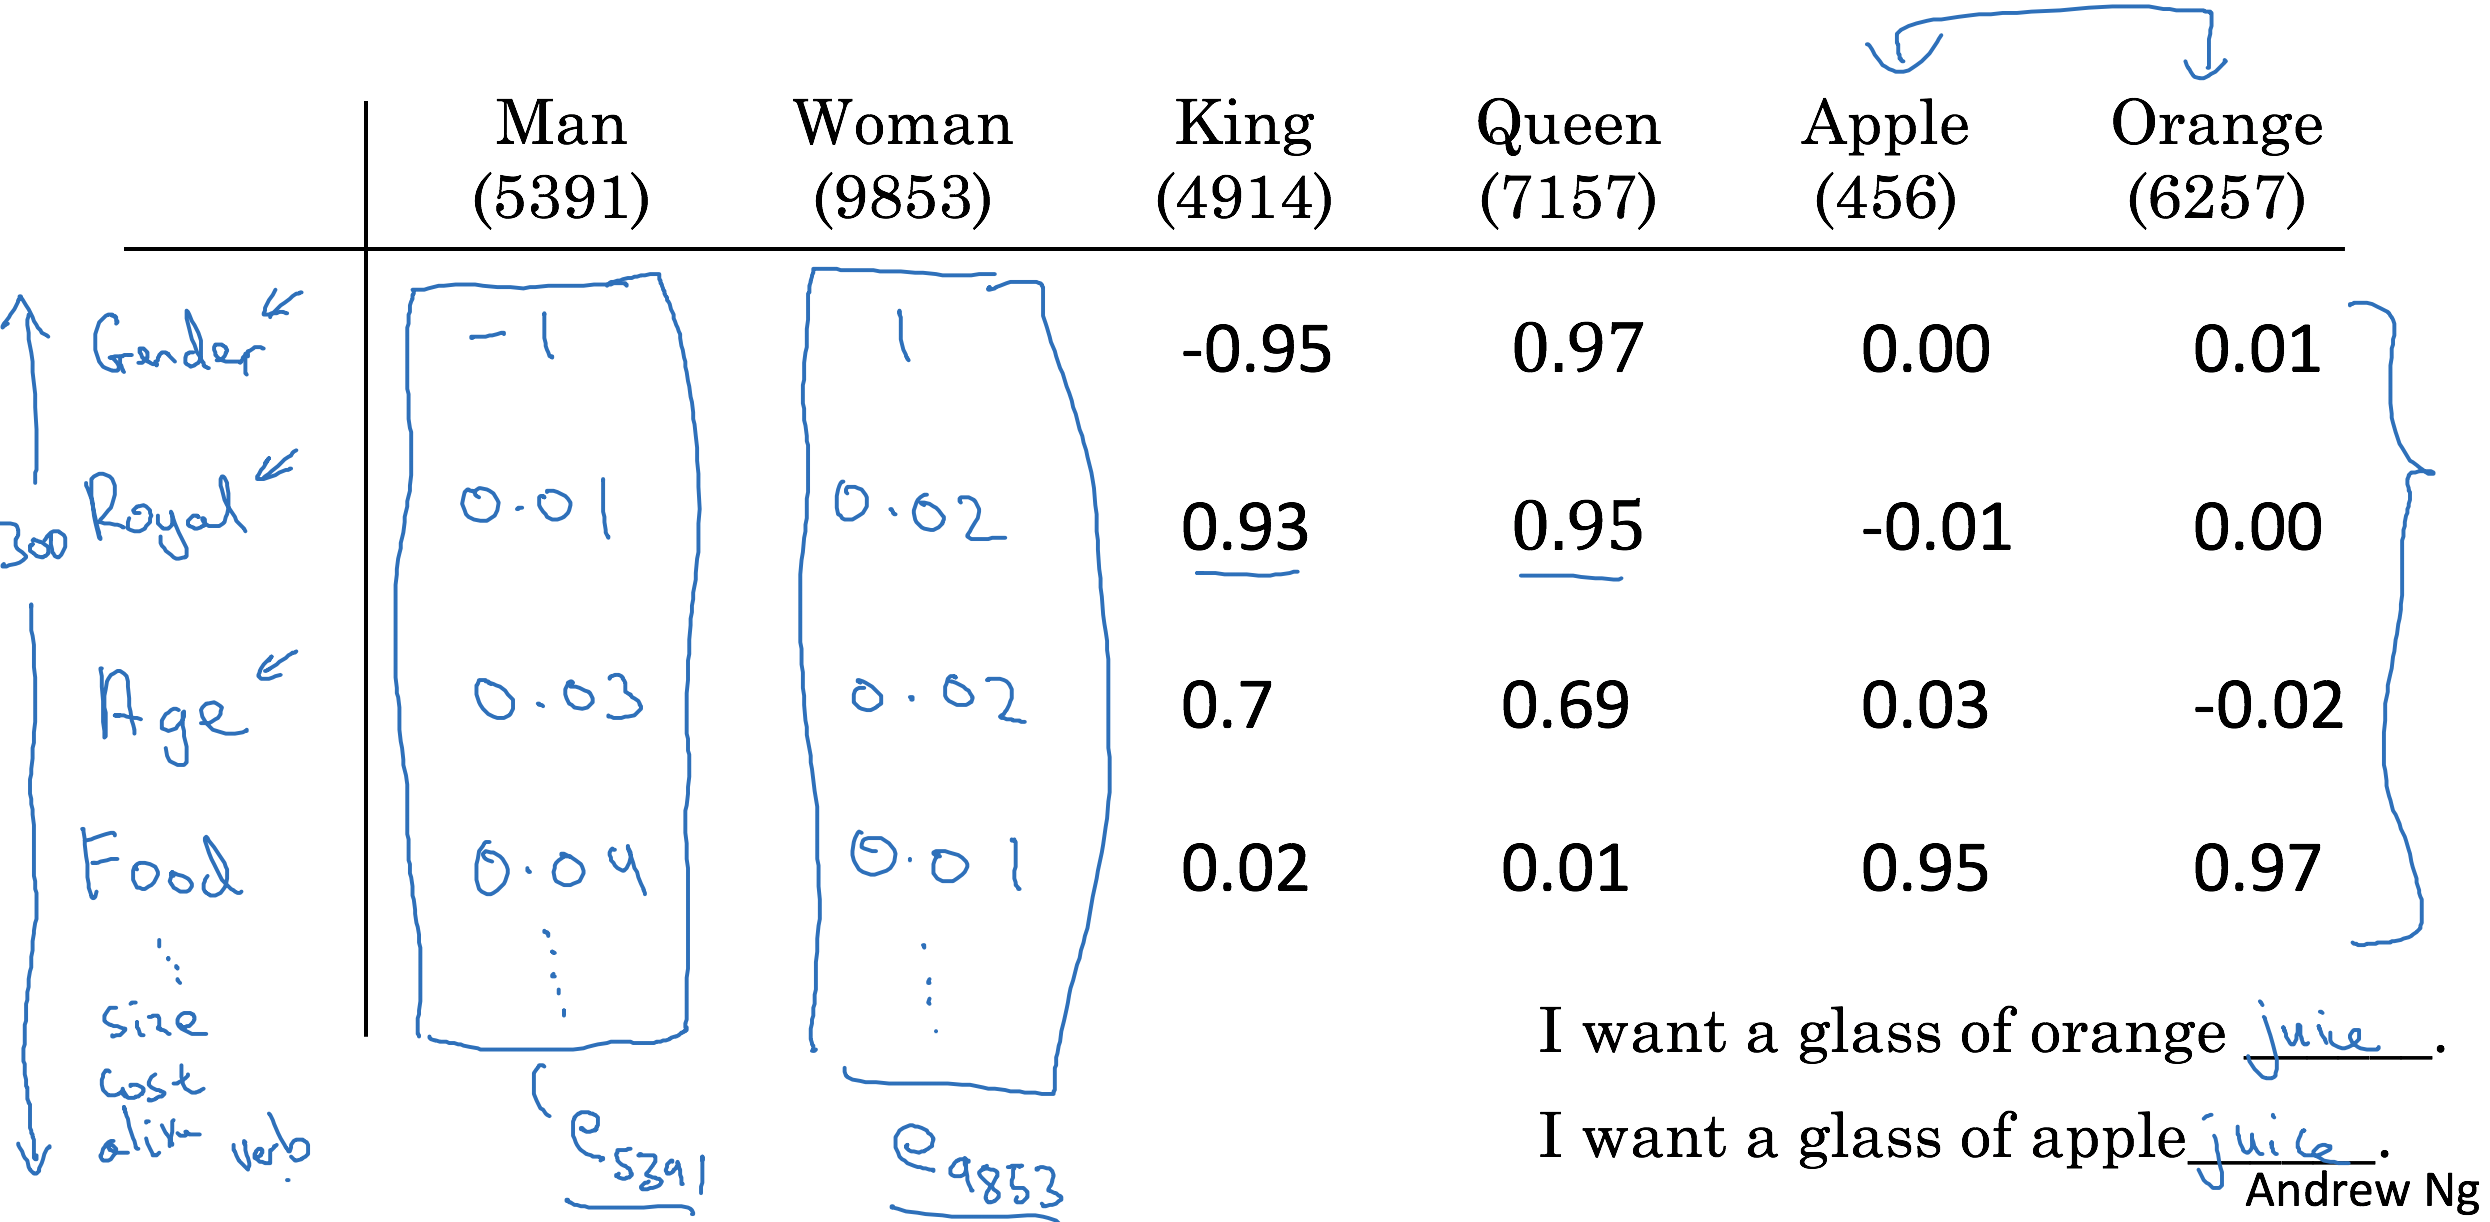
\includegraphics[scale=0.35]{Word_embedding}
\caption{Featurized representation: word embedding:}
\end{figure}
Instead, as in the picture, represent a word using high dimensional feature vector of values for each feature (e.g. gender, age, food). This allows to generalize better and learn a vectorized representation of words.

One of the algorithm, is \texttt{t-SNE}. A word is embeded in a 300 dimensional space, this is why it's called word embedding.

\subsubsection{Using word embeddings}

Transfer learning and word embeddings

\begin{enumerate}
    \item Learn word embeddings from large text corpus. (1-100B words).      (Or download pre-trained embedding online.)  
    \item Transfer embedding to new task with smaller training set.     (say, 100k words)
    \item Optional: Continue to finetune the word embeddings with new     data.
\end{enumerate}
Word embeddings (also called encoding)
\begin{itemize}
    \item  It has been useful for named entity recognition, for text summarization, for co-reference resolution, for parsing. These are all maybe pretty standard NLP tasks. 
    \item It has been less useful for language modeling, machine translation, especially if you're accessing a language modeling or machine translation task for which you have a lot of data just dedicated to that task.
\end{itemize}

\subsubsection{Properties of word embeddings}
Embeddings also help with analogies. Substracting the vectors for two words (say man and women, or kind and queen), capture the differences, in this case gender. The resulting vector should have approximately 0s everywhere except for the feature gender.

\begin{figure}[H]
\centering
\begin{equation*}
    e_{man} - e_{woman} \approx e_{king} - e_{?}
\end{equation*}
\caption{Analogies using word vectors}
\end{figure}

Find word w: 
\begin{equation}
  \text{arg } max_{w} \text{ Sim}(e_w, e_{king} - e_{man} + e_{woman})
\end{equation}

The mostly used similarity function is the \textbf{Cosine similarity}, cosine of the angle between two vectors:
\begin{equation}
  Sim(u, v) = \frac{u^T v}{\left|\left| u \right|\right|_2 \left|\left|v\right|\right|_2}
\end{equation}
It;s also possible to use the \textbf{Euclidean} distance, which is used most for dis-similarity.

\subsubsection{Embedding matrix}
Let's start to formalize the problem of learning a good word embedding. When you implement an algorithm to learn a word embedding, what you end up learning is an \textbf{embedding matrix}.

The goal is to lear the Embedding matrix \texttt{E}


\begin{figure}[H]
\centering
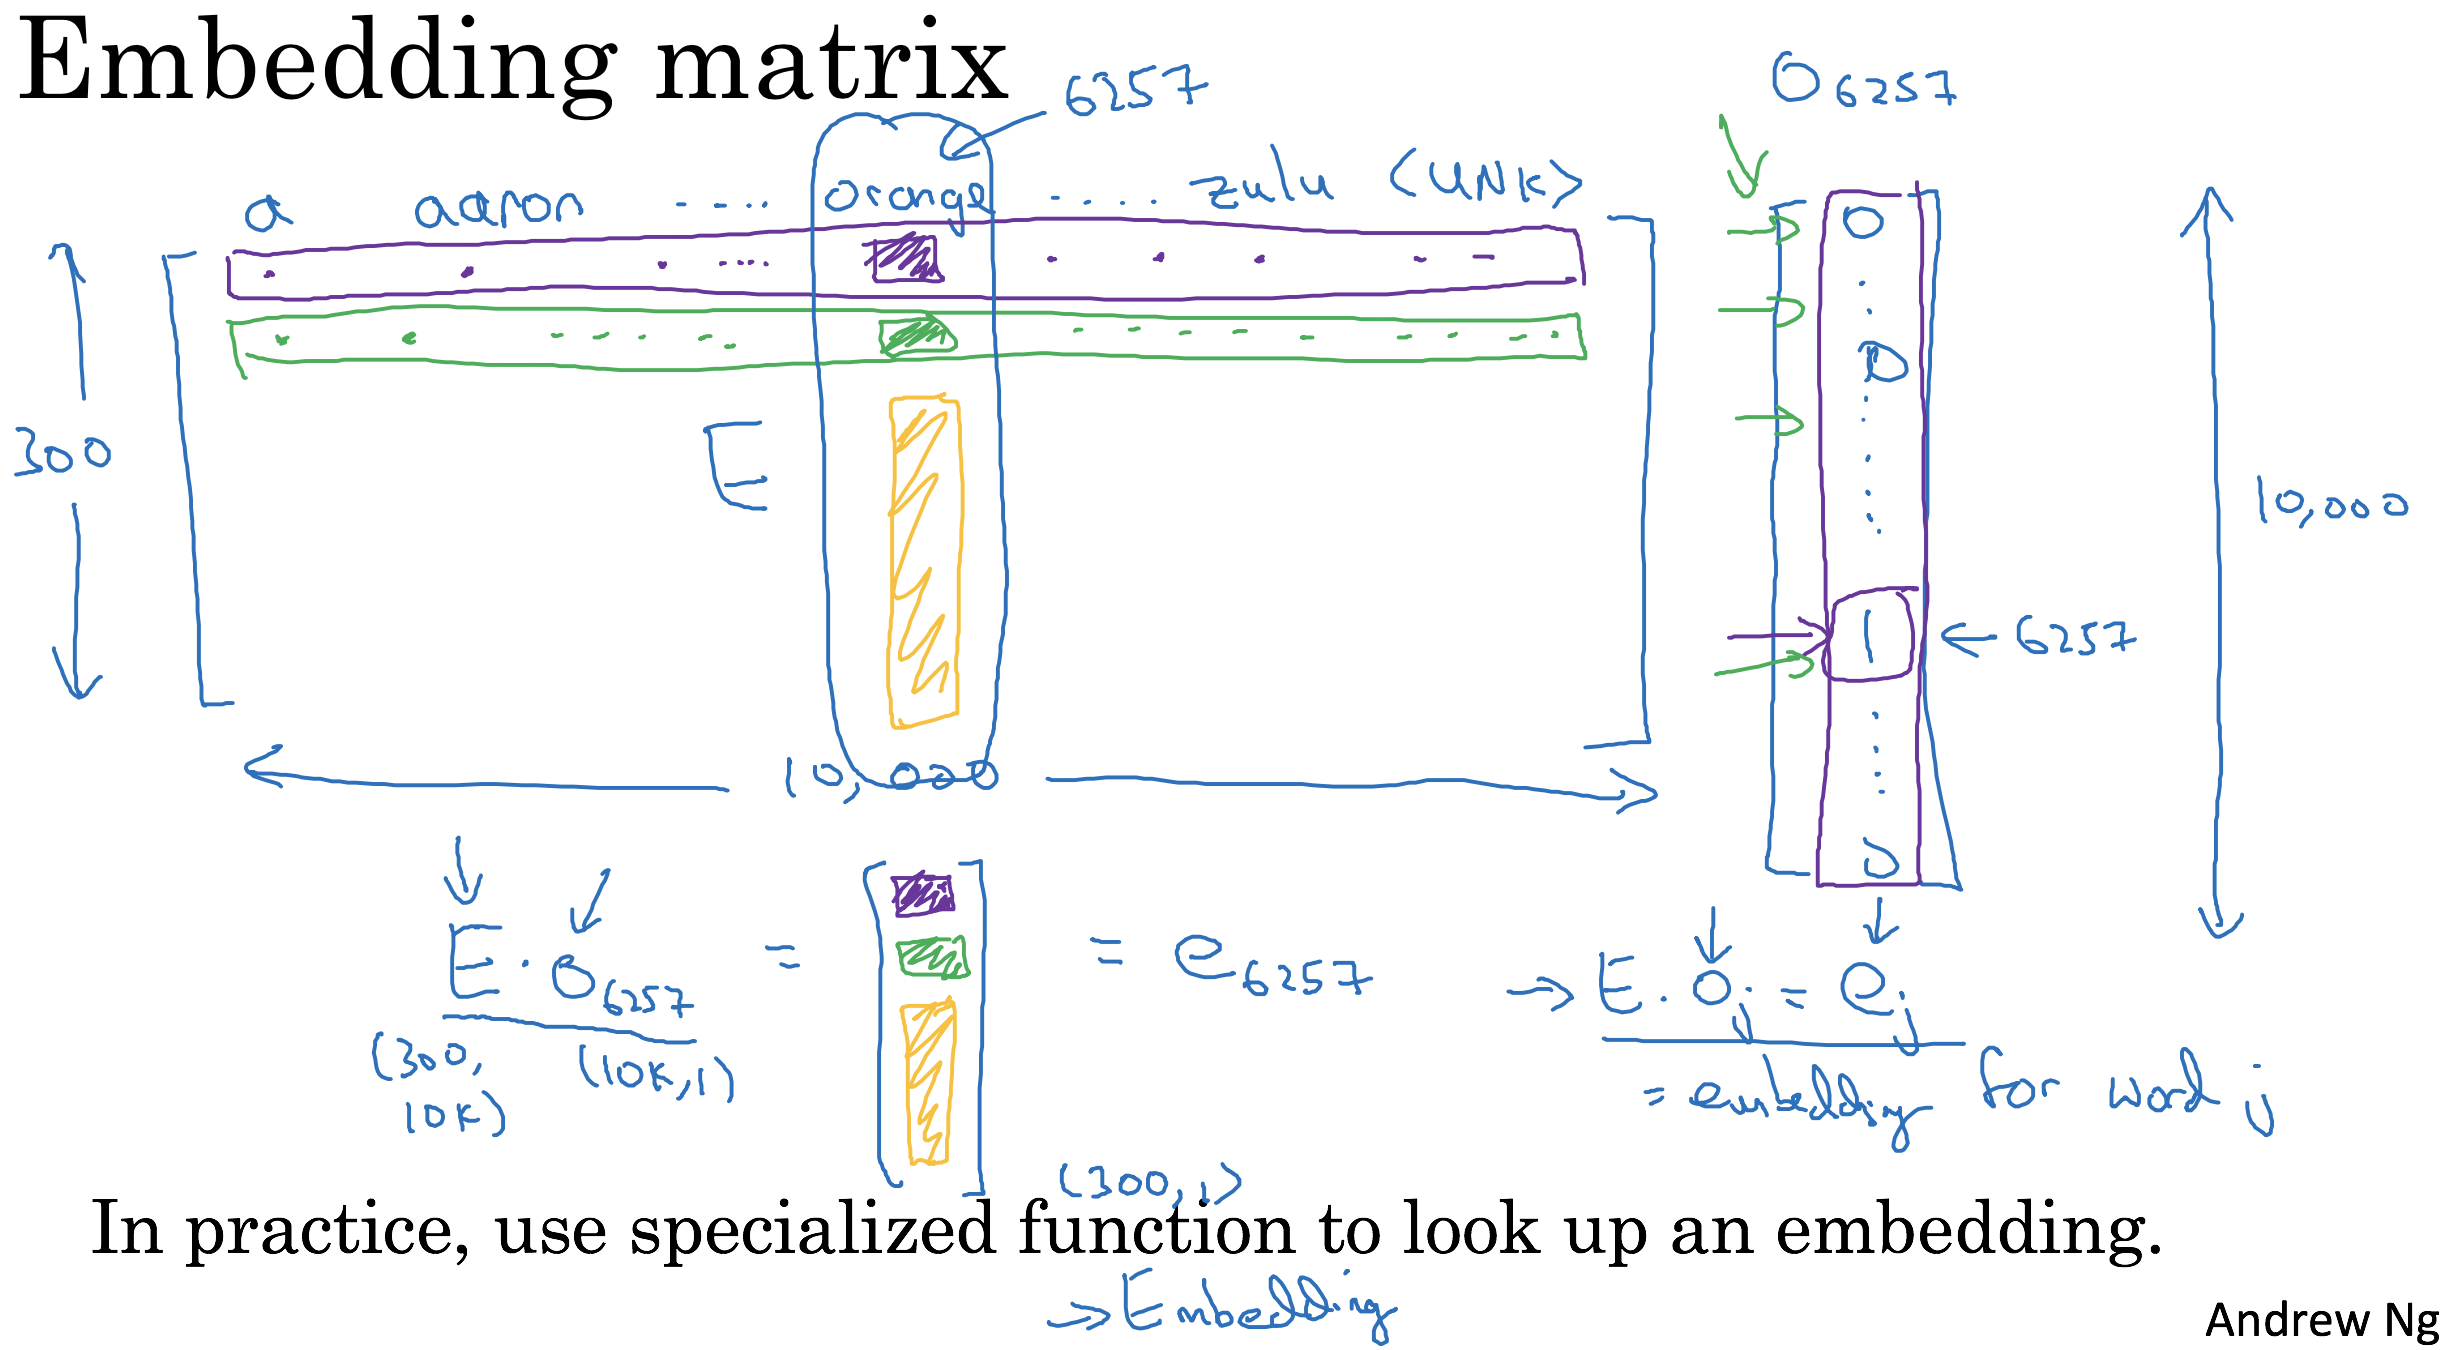
\includegraphics[scale=0.35]{Embedding_matrix}
\caption{Embedding matrix}
\end{figure}
The multiplication of $E * O_{6257}$ is computation expensive as this $O$ vector is one-hot vector all zeros but at the row for word 'Orange'. In practice we sue a specialized function to lookup an embedding, i.e. the columns that corresponds to the word Orange.

\subsection{Learning Word Embeddings: Word2vec \& GloVe}
Algorithms for learning the Embedding matrix \texttt{E}. 

\subsubsection{Learning word embeddings}
The parameters that need to be learned by the algorith, are: \texttt{E}, $W^{<1>}$, $b^{<1>}$.

\begin{figure}[H]
\centering
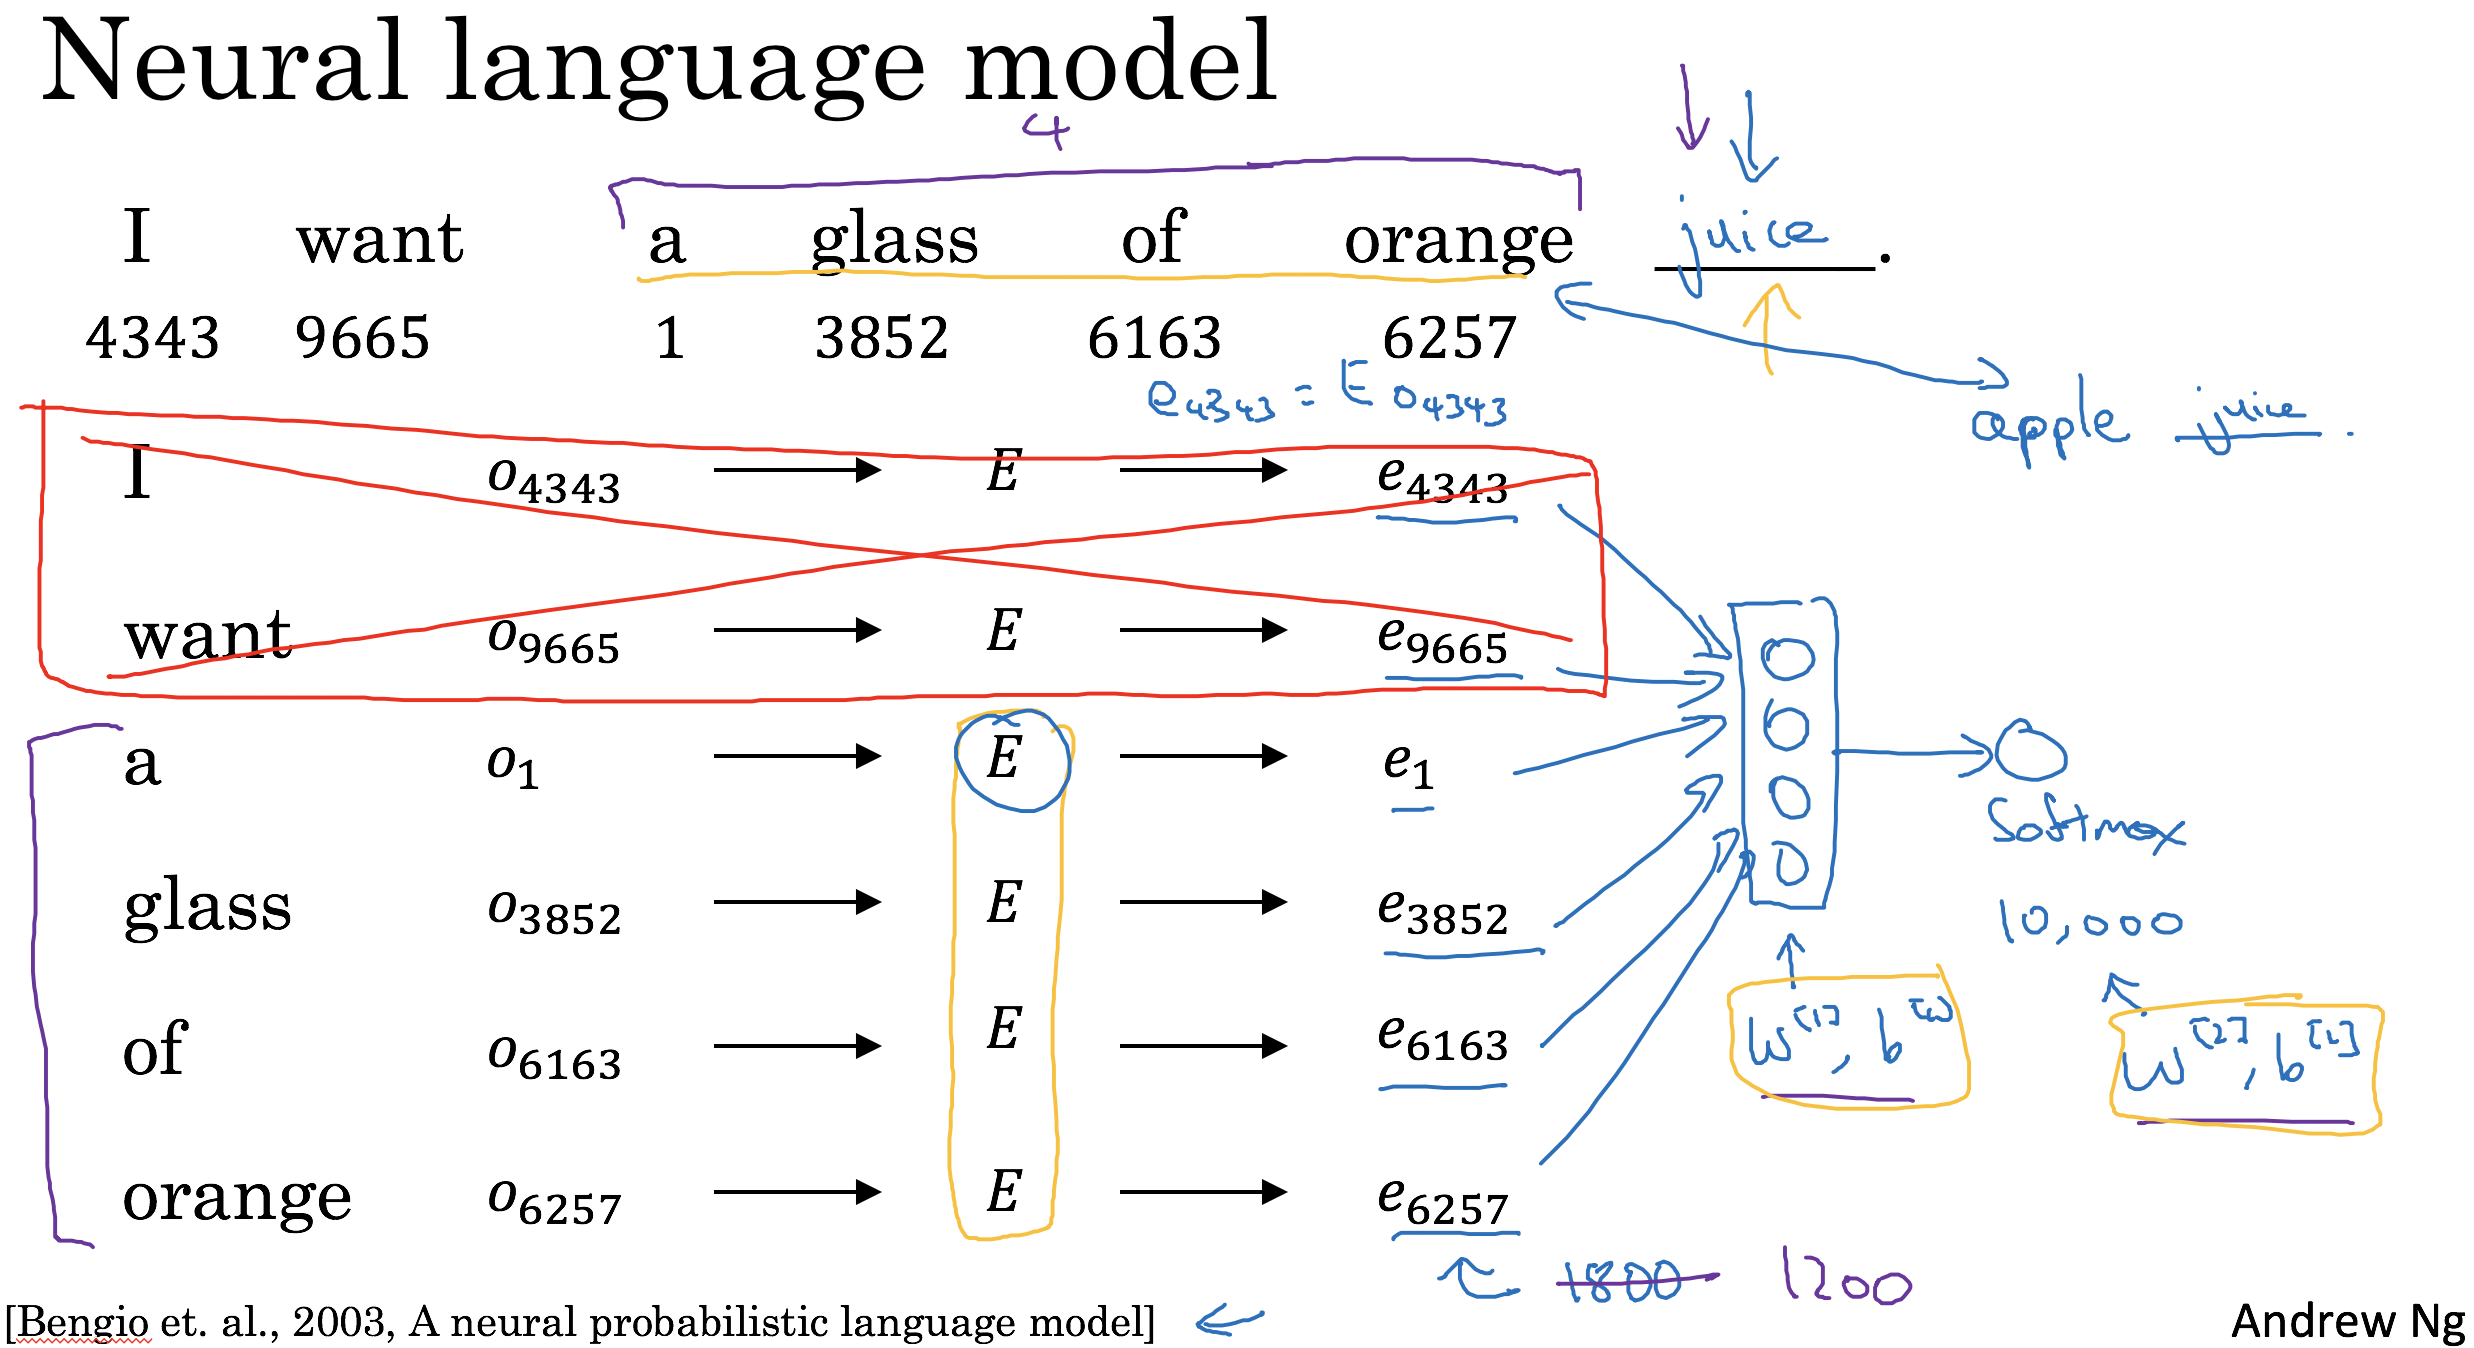
\includegraphics[scale=0.35]{Learning_word_embedding}
\caption{Learning word embedding}
\end{figure}
Context (the last three allows to learn embedding): 
\begin{itemize}
    \item last 4 words in the sentence,
    \item 4 words on left and right,
    \item last 1 word,
    \item nearby word.
\end{itemize}

\begin{quote}
    In the next video, you'll see how using even simpler context and even simpler learning algorithms to mark from context to target word, can also allow you to learn a good word embedding.
\end{quote}

\subsubsection{Word2Vec}
A simple algorithm with efficient computation.

Model
Vocab size = 10,000.
Content c x="orange" (word index: 6257) $==>$ Traget t y="juice" (word index: 4834)
\begin{equation*}
o_c -> E -> e_c = E*o_c -> o = softmax(e_c) -> \hat{y}
\end{equation*}

Softmax:
$\theta_t$ parameter associated with ouput t.
\begin{equation*}
  p(t | c) = \frac{\exp^{\theta^T_t e_c}}{\sum^{10000}_{j=1} \exp^{\theta^T_j e_c}}
\end{equation*}

Loss function:
\begin{equation*}
  \mathcal{L}(\hat{y}, y) = - \sum^{10000}_{i=1} y_i \log \hat{y}_i
\end{equation*}

Primary problem of this model is the computation speed, as you have to carry the sum of 10k in the softmax. One way to improve this is by using \textbf{Hierarchical Softmax} that gives you $log |v|$.

Different heuristics can be used to build the tree, to have common words in the top of the tree so that you can access them in few steps, while less common words are burried deep in the tree.

To sample the context c, you can sample randomly from your corpus, but you can heuritics so that $P(c)$ for sampling is not uniform, you don't want to have same probability for frequent words against uncommon words.

\subsubsection{Negative Sampling}
Defining a new supervised learning problem:

To generate the training set: 
\begin{enumerate}
    \item pick a context word (say orange) and a target word (say juice), then gives this row (e.g. orange juice) label 1.
    \item For k times, take same context word, then pick random word from dictionnary (e.g. of, the, book, etc.) and label all of them with 0. i.e. negative examples.
    \item Then, the supervised learning algorithm, will take X (context and target word) and try to predict the output label y.
\end{enumerate}
To choose K, it can be from 5 to 20, for lagest dataset chose smaller values (2 to 5).

\begin{figure}[H]
\centering
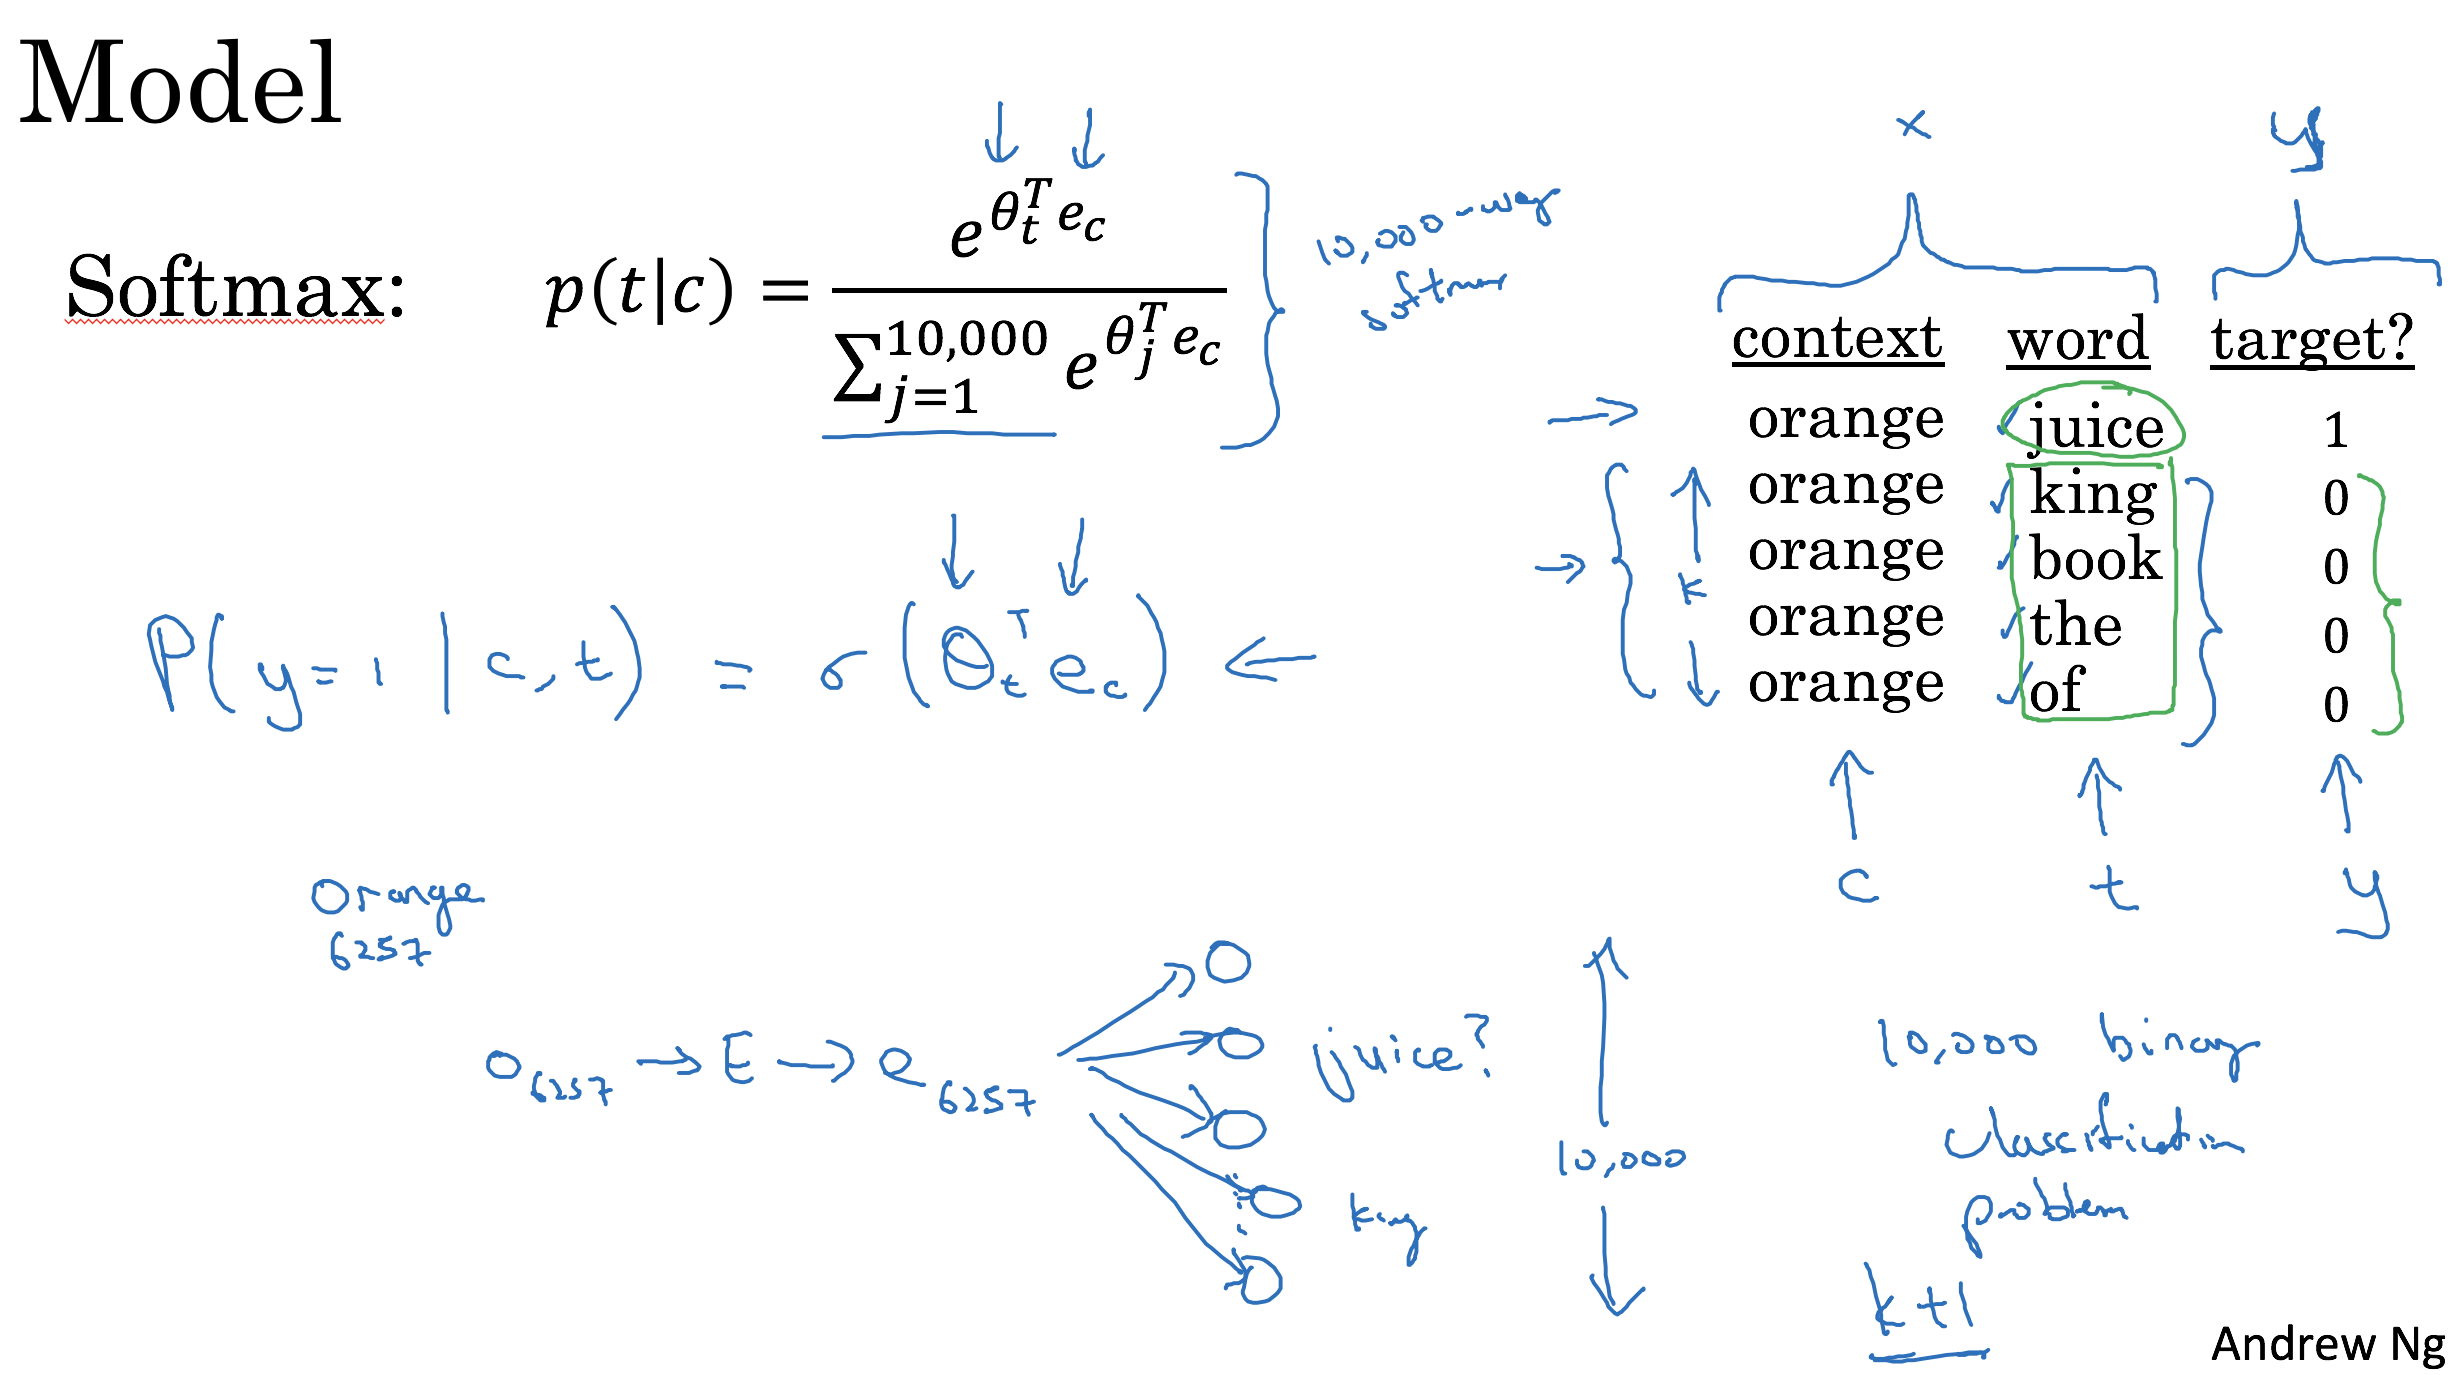
\includegraphics[scale=0.35]{Negative_Sampling_model}
\caption{Model of the supervised logistic regression}
\end{figure}

So think of this as having 10,000 binary logistic regression classifiers, but instead of training all 10,000 way Softmax on every iteration, we're only going to train five of them. We're going to train the one responding to the actual target word we got and then train 4 randomly chosen negative examples. This in case $k == 4$.


One word to sample the words (i.e. $P(w_i)$) for the negative samples is with words distribution but you will endup with common words like a, the, of. An alternative is to use the frequency $f$:
\begin{equation*}
    P(w_i) = \frac{f(w_i)^{3/4}}{\sum^{10000}_{j-1} f(w_j)^{3/4}}
\end{equation*}


\subsubsection{GloVe word vectors}

GloVe (global vectors for word representation), having Context c and taget t:
\begin{equation*}
    X_{ij} = \text{\# times i appears in context of j}
\end{equation*}

Model: GloVe tries to optimize the following:

\begin{equation*}
\text{mimimize} \sum^{10000}_{i=1} \sum^{10000}_{j=1} f(X_{ij}) (\theta^{T}_{i} e_{j} + b_i + b_j' - \log X_{ij})^2
\end{equation*}

\begin{itemize}
    \item $f(X_{ij}$ is a weithing term is 0 if $X_{ij} = 0$, it is used to avoid calculating log of 0.
    \item $\theta_i$, $\theta_j$ are symmetric
    \item $e^{(final)}_w = \frac{e_w + \theta_w}{2}$
\end{itemize}
The features detected by this algorithm are possible be non interpretable by humans, i.e. not just gender, age. But rather the learned features can be a combinations of say gender and age, etc.

\subsection{Applications using Word Embeddings}
\subsubsection{Sentiment Classification}
\begin{quote}
If you train this algorithm, you end up with a pretty decent sentiment classification algorithm and because your word embeddings can be trained from a much larger data set, this will do a better job generalizing to maybe even new words now that you'll see in your training set, such as if someone else says, "Completely absent of good taste, good service, and good ambiance" or something, then even if the word "absent" is not in your label training set, if it was in your 1 billion or 100 billion word corpus used to train the word embeddings, it might still get this right and generalize much better even to words that were in the training set used to train the word embeddings but not necessarily in the label training set that you had for specifically the sentiment classification problem. So that's it for sentiment classification, and I hope this gives you a sense of how once you've learned or downloaded from online a word embedding, this allows you to quite quickly build pretty effective NLP systems. 
\end{quote}
 

\begin{figure}[H]
\centering
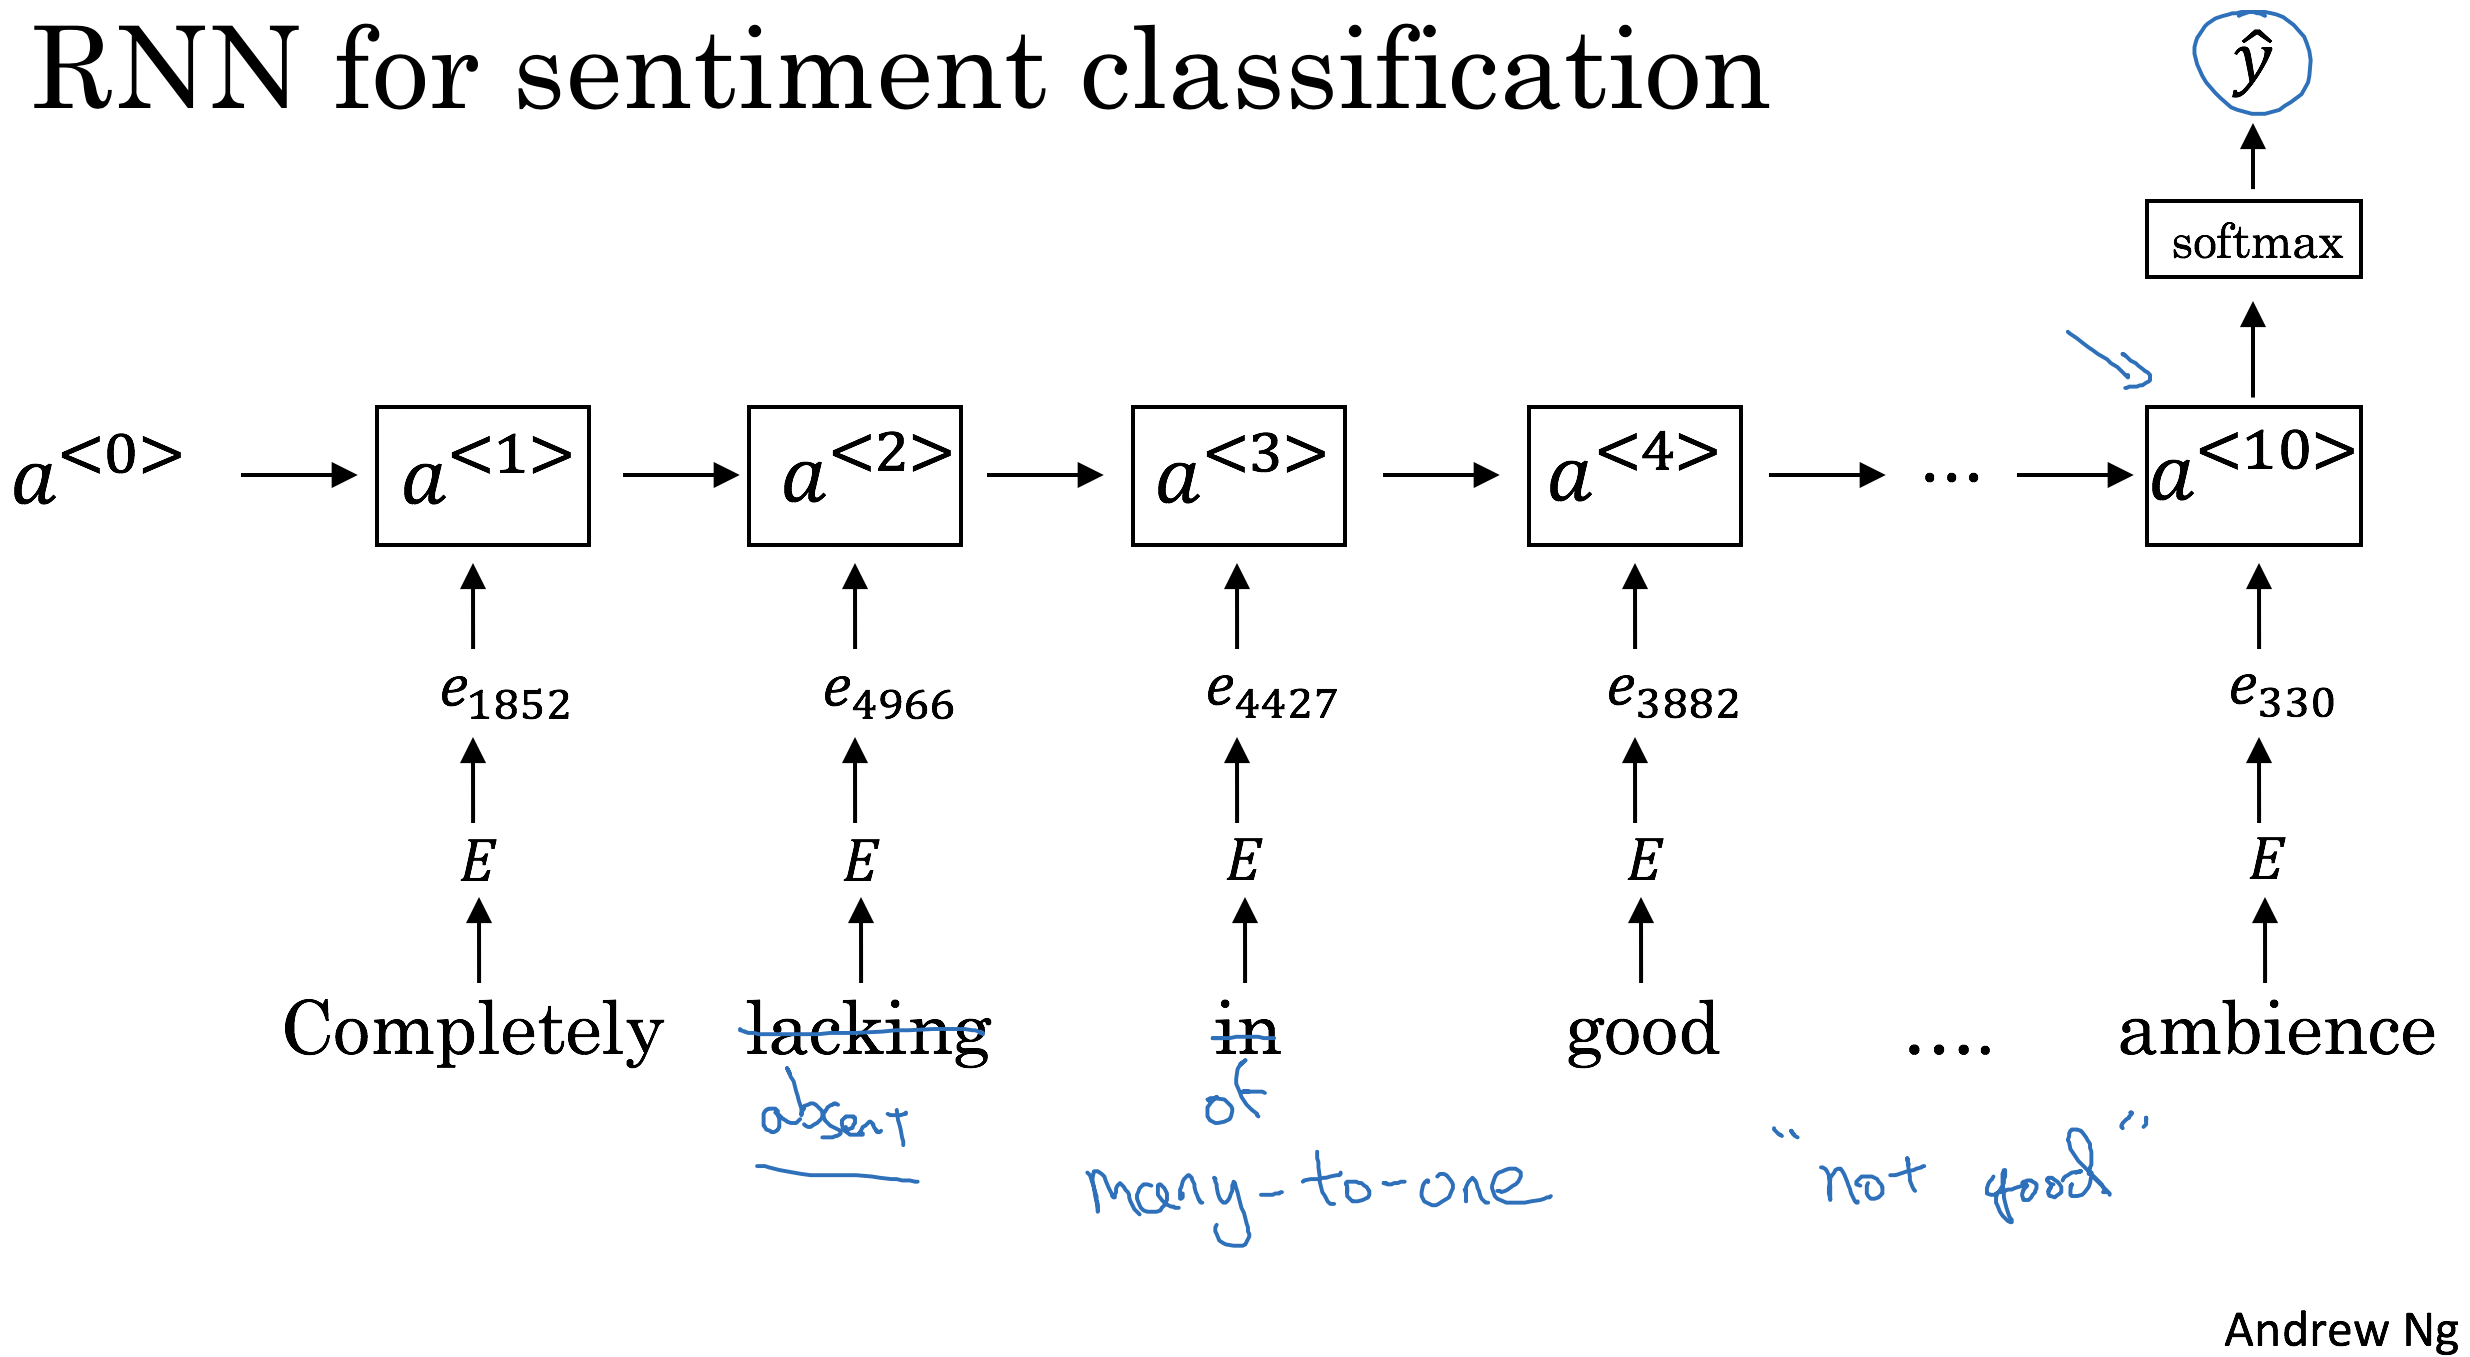
\includegraphics[scale=0.35]{RNN_sentiment_analysis}
\caption{RNN for sentiment analysis}
\end{figure}

\subsubsection{Debiasing word embeddings}
Some of the ideas of dimishing bias. In this case, it's about gender, ethnicity bias. Word embeddings can reflect the gender, ethnicity, age, sexual orientation, and other biases of the text used to train the model. You want wordds like Doctor to be gender neutral.

First step, Identifying bias direction:
\begin{itemize}
    \item $e_{he} - e_{she}$
    \item $e_{male} - e_{femal}$
    \item ...
\end{itemize}
Then average them (or simialar idea to PCA), to detect bias direction.
Second step, neutralize: for every word that is not definitional (not words like grandmother which is female, grandfather which is male), project to get rid of bias
Third step, equalize pairs, e.g. grandmother/girl should be equalized to grandfather/boy.

To decide fo what words are definitial, a linear classifier can tell you what words can be classified as definitional vs. not.

\begin{figure}[H]
\centering
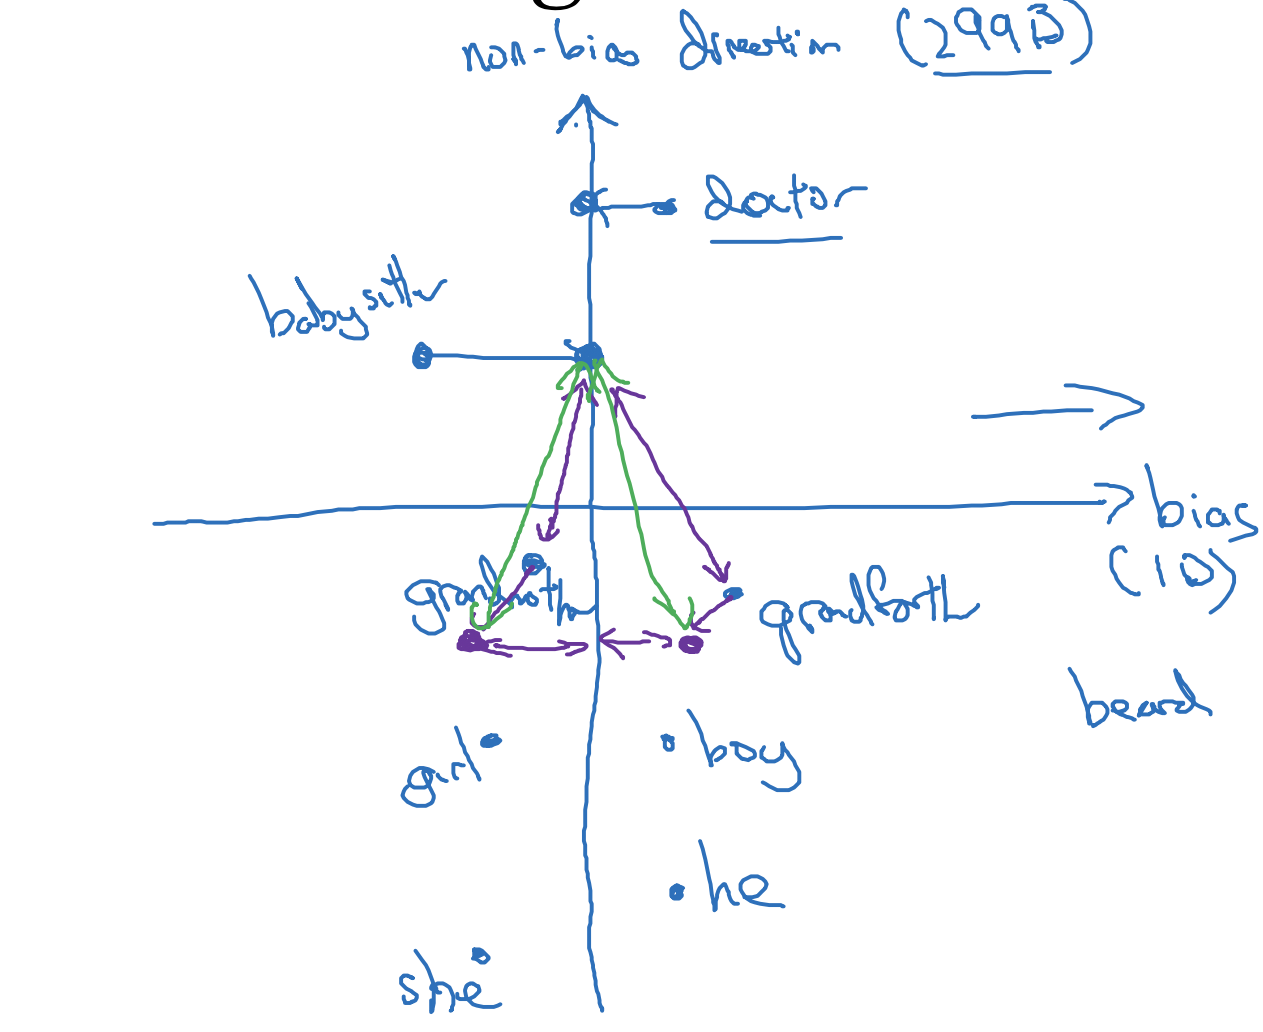
\includegraphics[scale=0.35]{Word_embeddings_Bias}
\caption{Addressing bias in word embeddings}
\end{figure}

\subsection{Practice questions}
\subsubsection{QUIZ - Natural Language Processing \& Word Embeddings}
\textbf{1.} Suppose you learn a word embedding for a vocabulary of 10000 words. Then the embedding vectors should be 10000 dimensional, so as to capture the full range of variation and meaning in those words.
\begin{itemize}
    \item True
    \item False (X) The dimension of word vectors is usually smaller than the size of the vocabulary. Most common sizes for word vectors ranges between 50 and 400.
\end{itemize}
\textbf{2.} What is t-SNE?
\begin{itemize}
    \item A linear transformation that allows us to solve analogies on word vectors
    \item A non-linear dimensionality reduction technique (X 2)
    \item A supervised learning algorithm for learning word embeddings (X 1) No
    \item An open-source sequence modeling library
\end{itemize}
\textbf{3.} Suppose you download a pre-trained word embedding which has been trained on a huge corpus of text. You then use this word embedding to train an RNN for a language task of recognizing if someone is happy from a short snippet of text, using a small training set.

Then even if the word “ecstatic” does not appear in your small training set, your RNN might reasonably be expected to recognize “I’m ecstatic” as deserving a label y = 1y=1.
\begin{itemize}
    \item True (X) Yes, word vectors empower your model with an incredible ability to generalize. The vector for "ecstatic would contain a positive/happy connotation which will probably make your model classified the sentence as a "1".
    \item False
\end{itemize}
\textbf{4.} Which of these equations do you think should hold for a good word embedding? (Check all that apply)
\begin{itemize}
    \item $e_{boy} - e_{girl} \approx e_{brother} - e_{sister}$ (X)
    \item $e_{boy} - e_{girl} \approx e_{sister} - e_{brother}$
    \item $e_{boy} - e_{brother} \approx e_{girl} - e_{sister}$ (X)
    \item $e_{boy} - e_{brother} \approx e_{sister} - e_{girl}$
\end{itemize}
\textbf{5.} Let $E$ be an embedding matrix, and let $o_{1234}$ be a one-hot vector corresponding to word 1234. Then to get the embedding of word 1234, why don’t we call $E * o_{1234}$ in Python?
\begin{itemize}
    \item It is computationally wasteful. (X) Yes, the element-wise multiplication will be extremely inefficient.
    \item The correct formula is $E^T* o_{1234}$
    \item This doesn’t handle unknown words (<UNK>).
    \item None of the above: calling the Python snippet as described above is fine.
\end{itemize}
\textbf{6.} When learning word embeddings, we create an artificial task of estimating $P(target \mid context)$. It is okay if we do poorly on this artificial prediction task; the more important by-product of this task is that we learn a useful set of word embeddings.
\begin{itemize}
    \item True (X)
    \item False
\end{itemize}
\textbf{7.} In the word2vec algorithm, you estimate $P(t \mid c)$, where $t$ is the target word and $c$ is a context word. How are $t$ and $c$ chosen from the training set? Pick the best answer.
\begin{itemize}
    \item $c$ and $t$ are chosen to be nearby words.
    \item $c$ is a sequence of several words immediately before $t$. (X 2)
    \item $c$ is the sequence of all the words in the sentence before $t$.
    \item $c$ is the one word that comes immediately before $t$. (X 1)
\end{itemize}
\textbf{8.} Suppose you have a 10000 word vocabulary, and are learning 500-dimensional word embeddings. The word2vec model uses the following softmax function:
\begin{equation*}
     P(t | c) = \frac{e^{\theta^T}_t e_c}{\sum^{10000}_{t'=1} e^{\theta^T}_{t'} e_c}
\end{equation*}
Which of these statements are correct? Check all that apply.
\begin{itemize}
    \item $\theta$ and $e_c$ are both 500 dimensional vectors. (X)
    \item $\theta_t$ and $e_c$ are both 10000 dimensional vectors.
    \item $\theta_t$ and $e_c$ are both trained with an optimization algorithm such as Adam or gradient descent. (X)
    \item After training, we should expect $\theta_t$ to be very close to $e_c$ when $t$ and cc are the same word.
\end{itemize}
\textbf{9.} Suppose you have a 10000 word vocabulary, and are learning 500-dimensional word embeddings.The GloVe model minimizes this objective:
\begin{equation*}
    min \sum^{10000}_{i=1} \sum^{10000}_{j=1} = f(X_{ij}) (\theta^{T}_{i} e_{j} + b_i + b_{j}' - \log X_{ij})^2
\end{equation*}
Which of these statements are correct? Check all that apply.
\begin{itemize}
    \item $\theta_i$ and $e_j$ should be initialized to 0 at the beginning of training.
    \item $\theta_i$ and $e_j$ should be initialized randomly at the beginning of training. (X)
    \item $X_{ij}$ is the number of times word i appears in the context of word j. (X)
    \item The weighting function $f(.)$ must satisfy $f(0) = 0$. (X) The weighting function helps prevent learning only from extremely common word pairs. It is not necessary that it satisfies this function.
\end{itemize}
\textbf{10.} You have trained word embeddings using a text dataset of $m_1$ words. You are considering using these word embeddings for a language task, for which you have a separate labeled dataset of $m_2$ words. Keeping in mind that using word embeddings is a form of transfer learning, under which of these circumstance would you expect the word embeddings to be helpful?
\begin{itemize}
    \item $m_1 >> m_2$ (X)
    \item $m_1 << m_2$
\end{itemize}